\begin{explanationbox}

    \textbf{\textcolor{CExplanation}{先从初中最熟悉的图形入手}}

    \textbf{场景一：普通三角形——不需要知道斜边有多长，也能求面积。}

    设 $A(0,2)$、$B(4,6)$、$P(2,0)$，$M$ 为 $AB$ 的中点。
    由中点公式，
    \[
        M\left(\frac{0+4}{2},\frac{2+6}{2}\right)=(2,4).
    \]
    点 $P,M$ 的横坐标同为 $2$，所以 $PM$ 竖直，$PM=4$。
    % 初中衔接：精确坐标 A(0,2), B(4,6), P(2,0), M(2,4)
\begin{center}
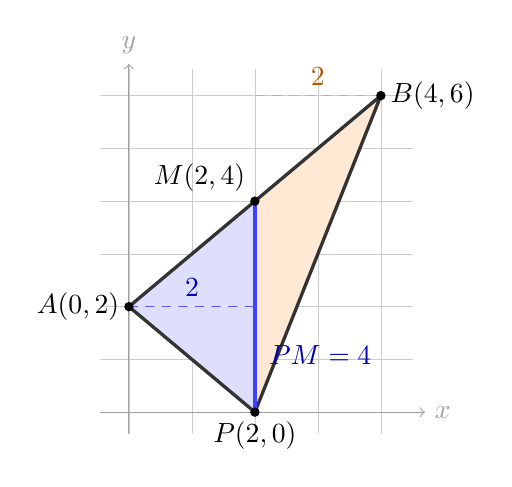
\begin{tikzpicture}[x=0.8cm,y=0.67cm, line cap=round, line join=round]
  \draw[gray!40,step=1,very thin] (-0.45,-0.4) grid (4.5,6.5);
  \draw[->,gray!75] (-0.45,0)--(4.7,0) node[right] {$x$};
  \draw[->,gray!75] (0,-0.4)--(0,6.6) node[above] {$y$};
  \coordinate (A) at (0,2);
  \coordinate (B) at (4,6);
  \coordinate (P) at (2,0);
  \coordinate (M) at (2,4);
  \fill[blue!13] (P)--(A)--(M)--cycle;
  \fill[orange!17] (P)--(M)--(B)--cycle;
  \draw[very thick,black!80] (P)--(A)--(B)--cycle;
  \draw[very thick,blue!75] (P)--(M);
  \draw[dashed,blue!65] (A)--(0,2)--(2,2);
  \draw[dashed,orange!75] (B)--(2,6);
  \fill (A) circle (1.7pt) node[left] {$A(0,2)$};
  \fill (B) circle (1.7pt) node[right] {$B(4,6)$};
  \fill (P) circle (1.7pt) node[below] {$P(2,0)$};
  \fill (M) circle (1.7pt) node[above left] {$M(2,4)$};
  \node[blue!70!black,anchor=south] at (1,2.0) {$2$};
  \node[orange!70!black,anchor=south] at (3.0,6.0) {$2$};
  \node[blue!70!black,right] at (2.07,1.08) {$PM=4$};
\end{tikzpicture}
\end{center}

    点 $A$ 到直线 $PM$ 的\textbf{水平距离}是 $|0-2|=2$；
    点 $B$ 到这条直线的\textbf{水平距离}是 $|4-2|=2$。
    把三角形分成 $\triangle PAM$ 和 $\triangle PMB$，分别应用初中的
    “底乘高除以二”：
    \[
    \begin{aligned}
        S_{\triangle PAB}
        &=S_{\triangle PAM}+S_{\triangle PMB}\\
        &=\frac12\times4\times2+\frac12\times4\times2
          =\boxed{8}.
    \end{aligned}
    \]
    \textbf{理解：}虽然 $AB$ 倾斜，$PM$ 并不垂直于 $AB$，
    仍然可以把 $PM$ 当作\textbf{两个小三角形共同的底边}。
    因为这时的高是左右两点到竖直直线的\textbf{水平距离}。

    \medskip
    \textbf{场景二：初中圆——从圆外一点作两条切线。}

    设 $P$ 是圆外一点，$PA,PB$ 分别切圆于 $A,B$，
    $O$ 为圆心，$M$ 为 $AB$ 的中点。
    % 初中衔接：圆心 O(0,0)、半径3、P(5,0)，真实切点 A(9/5,12/5), B(9/5,-12/5)
\begin{center}
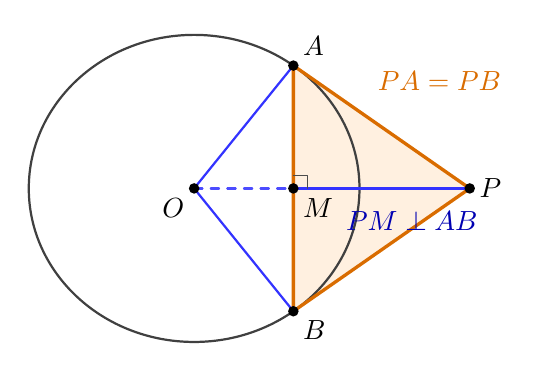
\begin{tikzpicture}[x=0.70cm,y=0.65cm,line cap=round,line join=round]
  \coordinate (O) at (0,0);
  \coordinate (P) at (5,0);
  \coordinate (A) at (1.8,2.4);
  \coordinate (B) at (1.8,-2.4);
  \coordinate (M) at (1.8,0);
  \fill[orange!12] (P)--(A)--(B)--cycle;
  \draw[thick,black!75] (O) circle (3);
  \draw[very thick,orange!85!black] (P)--(A)--(B)--cycle;
  \draw[blue!80,thick] (O)--(A) (O)--(B);
  \draw[blue!70,dashed,thick] (O)--(P);
  \draw[blue!80,very thick] (P)--(M);
  % Since AB is vertical and PM horizontal, their crossing is perpendicular.
  \draw[thin,black!70] (1.8,0.25)--(2.05,0.25)--(2.05,0);
  \fill (O) circle (1.9pt) node[below left] {$O$};
  \fill (P) circle (1.9pt) node[right] {$P$};
  \fill (A) circle (1.9pt) node[above right] {$A$};
  \fill (B) circle (1.9pt) node[below right] {$B$};
  \fill (M) circle (1.9pt) node[below right] {$M$};
  \node[orange!85!black] at (4.45,2.1) {$PA=PB$};
  \node[blue!70!black] at (3.95,-0.63) {$PM\perp AB$};
\end{tikzpicture}
\end{center}

    由\textbf{半径垂直于切线}，得 $OA\perp PA$、$OB\perp PB$。
    两个直角三角形 $\triangle OAP$、$\triangle OBP$ 中，
    $OP$ 是共同的斜边，$OA=OB$ 是半径，于是根据勾股定理，
    \[
        PA^2=OP^2-OA^2=OP^2-OB^2=PB^2.
    \]
    因为 $PA,PB$ 都是正的线段长度，得 $PA=PB$。
    所以 $\triangle PAB$ 是\textbf{等腰三角形}，
    从顶点 $P$ 到底边中点 $M$ 的中线也垂直于 $AB$，因而
    \[
        \boxed{S_{\triangle PAB}=\frac12 AB\cdot PM}
        \qquad\text{（这里 $PM$ 真的是 $AB$ 上的高）}.
    \]

    \textbf{场景三：换成抛物线——保留“两切线交于一点”的图形。}

    仍设切点为 $A,B$，切线交于 $P$，$M$ 为 $AB$ 中点。
    \textbf{相同点：}都要找“两切线交点 $P$、切点弦 $AB$、中点 $M$”。
    \textbf{不同点：}对 $x^2=2py$，能证明的是
    $x_P=x_M$，即 $PM$\textbf{平行于 $y$ 轴}；
    一般不能证明 $PA=PB$，也不能证明 $PM\perp AB$。
    因此不能照搬圆的“$AB\times PM/2$”，
    而要回到场景一的\textbf{分成两个小三角形}：
    \[
        \boxed{S_{\triangle PAB}
        =\frac12 PM\bigl(|x_1-x_P|+|x_2-x_P|\bigr)
        =\frac12 PM\,|x_1-x_2|}.
    \]
    最后一个等号成立的原因是
    $x_P=x_M=(x_1+x_2)/2$，所以 $x_P$ 恰好位于 $x_1,x_2$ 的中间。
    \textbf{这一步就是初中三角形面积与高中抛物线面积公式之间的桥梁。}

    \medskip
    \textbf{\textcolor{CExplanation}{进入高中结论}}


    \textbf{\textcolor{CExplanation}{一句话抓住本质}}

    \textbf{两切线交点 $P$ 正好位于底边 $AB$ 的中点 $M$ 的正下方。}
    这样就不用先求斜边 $AB$ 的长度、再求点到直线的距离；
    直接把 $PM$ 当成一条竖直的底边，利用水平距离求面积即可。

    \medskip

    \begin{center}
\begin{tikzpicture}[x=1.05cm,y=1.05cm,font=\small,>=Stealth]
\path (-2,-2.1) rectangle (9,3.6);
\coordinate (A) at (-1,.25); \coordinate (B) at (3,2.25);
\coordinate (P) at (1,-.75); \coordinate (M) at (1,1.25);
\coordinate (N) at (1,.25); \coordinate (H) at (.2,.85);
\fill[blue!12] (P)--(A)--(M)--cycle;
\fill[orange!20] (P)--(M)--(B)--cycle;
\draw[->,gray] (-1.8,0)--(3.8,0) node[right] {$x$};
\draw[->,gray] (0,-1.35)--(0,3.2) node[above] {$y$};
\draw[blue!70!black,thick,domain=-1.6:3.45,samples=100] plot (\x,{\x*\x/4});
\draw[gray!80,domain=-1.7:1.5] plot (\x,{-.5*\x-.25});
\draw[gray!80,domain=.7:3.4] plot (\x,{1.5*\x-2.25});
\draw[very thick] (A)--(B);
\draw[thick] (A)--(P)--(B);
\draw[orange!80!black,very thick] (P)--(M);
\foreach \pt/\pos in {B/above left,M/above left}
  \fill (\pt) circle (1.6pt) node[\pos] {$\pt$};
\fill (A) circle (1.6pt); \node[anchor=east] at (-1.3,-.35) {$A$};
\fill (P) circle (1.6pt); \node[anchor=west] at (1.4,-.65) {$P$};

\draw[orange!80!black,dashed] (1,-.9)--(1,2.7);
\draw[teal!80!black] (-1,.25)--(1,.25);
\draw[dashed,teal!80!black] (-1,.25)--(-1,-1.5) (1,-.9)--(1,-1.5);
\draw[<->,teal!80!black] (-1,-1.45)--(1,-1.45) node[midway,below] {$h_A$};
\draw[<->,teal!80!black] (1,2.25)--(3,2.25) node[midway,above] {$h_B$};
\draw (1,.4)--(.85,.4)--(.85,.25);
\draw (1,2.1)--(1.15,2.1)--(1.15,2.25);

\node[anchor=north west,align=left,text width=4.7cm] at (4.1,3.1) {\textbf{同底 $PM$，水平作高}\\[8pt]
$h_A=|x_1-x_P|$\\[5pt]
$h_B=|x_2-x_P|$\\[8pt]
$h_A+h_B=|x_2-x_1|$\\[8pt]
$S_{PAM}+S_{PMB}$\\[4pt]
$\quad=\dfrac12 PM(h_A+h_B)$\\[8pt]
水平高落在直线 $PM$ 上，\\不必落在线段 $PM$ 内。};
\end{tikzpicture}
\end{center}

    图中蓝、橙两块共用竖直底边 $PM$，水平高分别为 $h_A,h_B$。
    它们相加等于 $|x_1-x_2|$，所以
    \[
        S=\frac12 PM(h_A+h_B)=\frac12 PM\,|x_1-x_2|.
    \]
    \medskip
    \textbf{\textcolor{CExplanation}{为什么横坐标会出现“平均数”？}}

    过切点 $A(x_1,y_1)$ 的切线为
    $x_1x=p(y+y_1)$；过 $B$ 的切线为 $x_2x=p(y+y_2)$。
    因为 $P$ 同时在这两条切线上，
    \[
        x_1x_P=p(y_P+y_1),\qquad
        x_2x_P=p(y_P+y_2).
    \]
    \textbf{相减的目的：}消去两式里相同的 $py_P$，从而求出交点横坐标。
    \[
    \begin{aligned}
        (x_1-x_2)x_P
        &=p(y_1-y_2)\\
        &=p\frac{x_1^2-x_2^2}{2p}\\
        &=\frac{(x_1-x_2)(x_1+x_2)}{2}.
    \end{aligned}
    \]
    消去非零的 $x_1-x_2$，就得到 $x_P=(x_1+x_2)/2$。
    \textbf{几何意义：}顶点恰好落在经过底边中点的竖直线上。

    \medskip
    \par\noindent\begin{minipage}{\linewidth}
    \textbf{\textcolor{CExplanation}{为什么面积中是“三次方”？}}

    中点 $M$ 和顶点 $P$ 的纵坐标分别是
    \end{minipage}\par
    \[
        y_M=\frac{x_1^2+x_2^2}{4p},\qquad
        y_P=\frac{x_1x_2}{2p}.
    \]
    因此
    \[
        PM=y_M-y_P
        =\frac{x_1^2+x_2^2-2x_1x_2}{4p}
        =\frac{(x_1-x_2)^2}{4p}.
    \]
    \textbf{几何意义：}两个切点在水平方向分得越开，竖直中线的长度
    按“横坐标差的平方”增加；而三角形的水平宽度又正比于“横坐标差”。
    面积把这两项相乘，于是出现三次方：
    \[
        \underbrace{\frac12}_{\text{面积系数}}
        \cdot\underbrace{|x_1-x_2|}_{\text{水平宽度}}
        \cdot\underbrace{\frac{(x_1-x_2)^2}{4p}}_{\text{竖直中线}}
        =\frac{|x_1-x_2|^3}{8p}.
    \]

    \medskip
    \textbf{\textcolor{CExplanation}{更进一步：中线为何被抛物线平分？}}


    \begin{center}
\begin{tikzpicture}[x=1.05cm,y=1.05cm,font=\small,>=Stealth]
\path (-2,-2.1) rectangle (9,3.6);
\coordinate (A) at (-1,.25); \coordinate (B) at (3,2.25);
\coordinate (P) at (1,-.75); \coordinate (M) at (1,1.25);
\coordinate (N) at (1,.25); \coordinate (H) at (.2,.85);
\fill[blue!12] (P)--(A)--(M)--cycle;
\fill[orange!20] (P)--(M)--(B)--cycle;
\draw[->,gray] (-1.8,0)--(3.8,0) node[right] {$x$};
\draw[->,gray] (0,-1.35)--(0,3.2) node[above] {$y$};
\draw[blue!70!black,thick,domain=-1.6:3.45,samples=100] plot (\x,{\x*\x/4});
\draw[gray!80,domain=-1.7:1.5] plot (\x,{-.5*\x-.25});
\draw[gray!80,domain=.7:3.4] plot (\x,{1.5*\x-2.25});
\draw[very thick] (A)--(B);
\draw[thick] (A)--(P)--(B);
\draw[orange!80!black,very thick] (P)--(M);
\foreach \pt/\pos in {B/above left,M/above left}
  \fill (\pt) circle (1.6pt) node[\pos] {$\pt$};
\fill (A) circle (1.6pt); \node[anchor=east] at (-1.3,-.35) {$A$};
\fill (P) circle (1.6pt); \node[anchor=west] at (1.4,-.65) {$P$};

\fill[blue!70!black] (N) circle (1.7pt) node[right] {$N$};
\draw[thick] (.88,-.25)--(1.12,-.25) (.88,.75)--(1.12,.75);

\node[anchor=north west,align=left,text width=4.7cm] at (4.1,3.1) {\textbf{平分的是线段 $PM$}\\[8pt]
$x_N=x_P=x_M$\\[8pt]
$y_N=\dfrac{(x_1+x_2)^2}{8p}$\\[10pt]
$PN=NM=\dfrac{PM}{2}$\\[8pt]
$P$ 是切线交点；\\$N$ 才是同横坐标的曲线点。\\[8pt]
两段曲线弧不据此等长。};
\end{tikzpicture}
\end{center}


    设 $N$ 与 $P,M$ 横坐标相同且在抛物线上，则
    \[
        y_N=\frac{((x_1+x_2)/2)^2}{2p}
        =\frac{(x_1+x_2)^2}{8p}.
    \]
    另一方面，线段 $PM$ 中点的纵坐标是
    \[
        \frac{y_P+y_M}{2}
        =\frac{\dfrac{x_1x_2}{2p}+\dfrac{x_1^2+x_2^2}{4p}}2
        =\frac{(x_1+x_2)^2}{8p}=y_N.
    \]
    所以 $N$ 正是 $PM$ 的中点。
    \textbf{注意：}这里说的是\textbf{线段 $PM$ 的中点}，不是说抛物线弧长被平分。

    \medskip
    \textbf{\textcolor{CExplanation}{画图与解题时的识别信号}}
    \begin{itemize}[leftmargin=*, itemsep=0.4em, topsep=0.35em]
        \item 题目出现“抛物线上两点的切线交于一点”：优先想切线点式及切点弦。
        \item 题目问面积：先找底边中点 $M$，再找竖直线段 $PM$，不要一开始就算斜边和点到斜线的距离。
        \item 题目已知切线交点 $P(x_0,y_0)$：先看 $x_0^2-2py_0$ 的正负，以判断能否作出两条不同的切线。
        \item 题目已知面积：只能先反求 $|x_1-x_2|$，不能仅凭面积确定两个切点各自的横坐标。
    \end{itemize}
\end{explanationbox}
